%% LaTeX Beamer presentation template (requires beamer package)
%% see http://bitbucket.org/rivanvx/beamer/wiki/Home
%% idea contributed by H. Turgut Uyar
%% template based on a template by Till Tantau
%% this template is still evolving - it might differ in future releases!

\documentclass{beamer}

\mode<presentation>
{
%\usetheme{Warsaw}
%\usetheme{Madrid}
\usetheme{Rochester}
%\usetheme{Singapore}

\setbeamercovered{transparent}
}

\usepackage[portuguese]{babel}
\usepackage[utf8]{inputenc}


% font definitions, try \usepackage{ae} instead of the following
% three lines if you don't like this look
\usepackage{mathptmx}
\usepackage[scaled=.90]{helvet}
\usepackage{courier}


\usepackage[T1]{fontenc}


\title{Contratos REST robustos e leves}

\subtitle{uma abordagem em Design-by-Contract com NeoIDL}

% - Use the \inst{?} command only if the authors have different
%   affiliation.
%\author{F.~Author\inst{1} \and S.~Another\inst{2}}
\author{Lucas F. Lima\inst{1} \\Orientadores: Rodrigo Bonifácio\inst{2}, Edna
Canedo\inst{3}}


% - Use the \inst command only if there are several affiliations.
% - Keep it simple, no one is interested in your street address.
\institute[Universities of]
{
\inst{1}%
Departamento de Engenharia Elétrica -- Universidade de Brasília --
 UnB
\and
\inst{2}%
Departamento de Ciência da Computação -- Universidade de Brasília -- UnB\\ 
\and
\inst{3}%
Faculdade UnB Gama -- Universidade de Brasília -- UnB\\ 
 Brasília -- DF -- Brasil}

\date{WTDSoft 2015}


% This is only inserted into the PDF information catalog. Can be left
% out.
\subject{Talks}



% If you have a file called "university-logo-filename.xxx", where xxx
% is a graphic format that can be processed by latex or pdflatex,
% resp., then you can add a logo as follows:

\pgfdeclareimage[height=1cm]{university-logo}{UnB.jpg}
\logo{\pgfuseimage{university-logo}}



% Delete this, if you do not want the table of contents to pop up at
% the beginning of each subsection:
% \AtBeginSubsection[]
% {
% \begin{frame}<beamer>
% \frametitle{O problema}
% \tableofcontents[currentsection,currentsubsection]
% \end{frame}
% }

% If you wish to uncover everything in a step-wise fashion, uncomment
% the following command:

%\beamerdefaultoverlayspecification{<+->}
\usepackage{listings}

\lstdefinelanguage{NeoIDL}{
  sensitive = true, 
  keywords = {module, resource, enum, annotation, for, import, entity, path,
  @get, require, ensure, otherwise},
 %basicstyle=\normalfont\ttfamily,
    numbers=left,
    numberstyle=\scriptsize,
    stepnumber=1,
    numbersep=8pt,
    showstringspaces=false,
    breaklines=true,
    frame=top,
    %backgroundcolor=\color{background}
}

\begin{document}

\begin{frame}
\titlepage
\end{frame}

%\begin{frame}
%\frametitle{O problema}
%\tableofcontents
% You might wish to add the option [pausesections]
%\end{frame}


\section{Introdução} 

\subsection[Contextualização]{First Subsection Name}

\begin{frame}
\frametitle{O problema}

O uso do padrão REST para construção de WebServices é crescente no contexto do
desenvolvimento de soluções basedas em serviço.
\vskip0pt plus.5fill 
REST não dispõe de uma linguagem padrão para especificação de
contratos. Frente a isso, a NeoIDL (DSL) foi desenvolvida para ser uma
alternativa, caracterizada pela coesão e simplicidade em se compreender.
\vskip0pt plus.5fill 

\pause Por outro lado, a NeoIDL suporta apenas contratos fracos (\it{weak
contracts}), sem suporte a construções como pré e pós condições.
\vskip0pt plus.5fill


\end{frame}

\begin{frame}
\frametitle{NeoIDL - Arquitetura}

\begin{figure}[h]
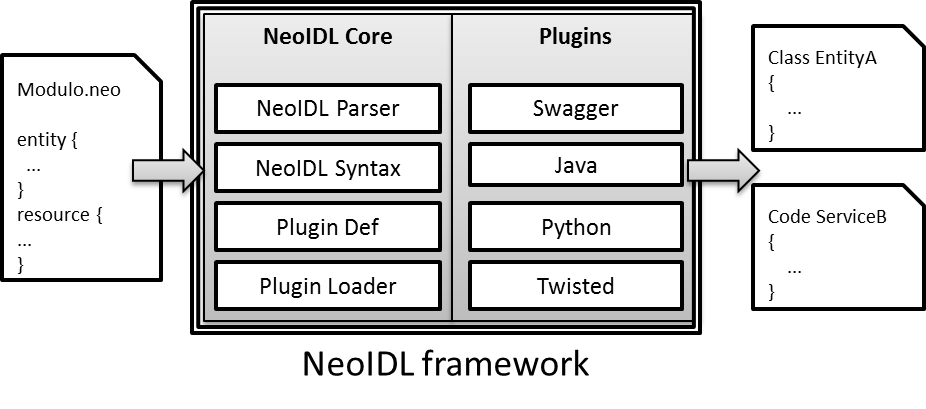
\includegraphics[width=10cm]{NeoIDLFrameworkArchitecture3.png}
%\caption{Comparação da redução em número de linhas (continuação)}\label{fig:02}
\end{figure}

\end{frame}


\begin{frame}
\frametitle{As contribuições}

\begin{itemize}  
  \item Introduzir o conceito de \alert{Design-by-Contract} no contexto da
  especificação de contratos REST para Computação Orientada a Serviços 
  \pause
  \vskip0pt plus.5fill
  \item Evolução da linguagem e \it{framework} NeoIDL para suportar \alert{novas
  construções}
  \vskip0pt plus.5fill
  \pause
  \item Avaliar a expressividade de contratos escritos na NeoIDL em
  contraponto a outra linguagem 
  \vskip0pt plus.5fill
  \pause
  \item Conduzir \alert{estudo empírico} para avaliar:
    \begin{itemize}
    \item Aptidão da NeoIDL para reuso de entidades
    \item Comprovar necessidades e benefícios do DbC em SOC
  \end{itemize}

\end{itemize}

\end{frame}


\begin{frame}
\frametitle{NeoIDL - exemplo de especificação}

\begin{figure}[htb]
\begin{tiny}
\lstinputlisting[language=NeoIDL,firstnumber=1]{getCharacters.tex}
\end{tiny}

getCharactersList - Marvel - especificado em NeoIDL
\end{figure}

\end{frame}


\begin{frame}
\frametitle{Design-by-contract - Contrato fraco e forte}

\begin{tabular}{|r|p{5cm}|}
\hline \multicolumn{2}{|c|}{Contrato fraco} \\ \hline
Pré condição: & True\\
Pós condição: & if empty(stack)\\ 
 & then thrown emptyException \\ 
 & else return top (stack) \\ \hline
\end{tabular}

\vskip0pt plus.5fill

\begin{tabular}{|r|p{5cm}|}
\hline \multicolumn{2}{|c|}{Contrato forte} \\ \hline
Pré condição: & not empty(stack) \\
Pós condição: & return top (stack) \\ \hline
\end{tabular}

\vskip0pt plus.5fill
Operação top()

\end{frame}


\begin{frame}
\frametitle{NeoIDL - exemplo de especificação com uso de DbC}

\begin{figure}[htb]
\begin{tiny}
\lstinputlisting[language=NeoIDL,firstnumber=1]{getCharactersDbc.tex}
\end{tiny}

getCharactersList - Marvel - especificado em NeoIDL

\label{lst:getCharacters-neo}
\end{figure}

\end{frame}

\begin{frame}
\frametitle{DbC - outro exemplo da literatura}

\begin{figure}[h]
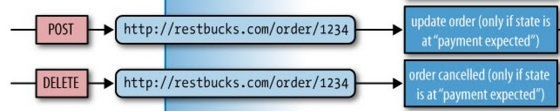
\includegraphics[width=7cm]{LojaCafeTrecho.jpg}
\end{figure}
\begin{center}
Cafeteria\footnote{Livro: REST in Practice - Hypermedia and System Architecture}
\end{center}
\vspace{-1cm}

\begin{figure}[htb]
\begin{tiny}
\lstinputlisting[language=NeoIDL,firstnumber=1]{deleteOrderCoffe.tex}
\end{tiny}


\label{lst:getCharacters-neo}
\end{figure}


\end{frame}

\subsection[Avaliação]{Avaliação} 

\begin{frame}
\frametitle{Prova de conceito - Twisted	}


\begin{figure}[h]
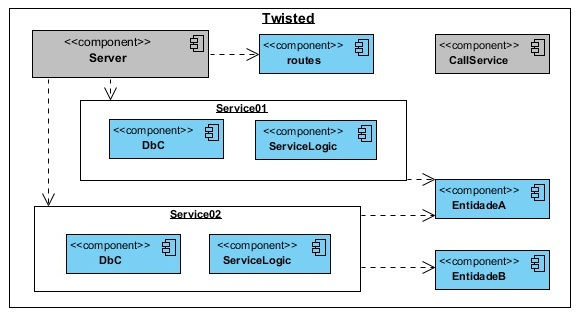
\includegraphics[width=8.5cm]{DigramaComponentesTwisted.jpg}
\end{figure}


\end{frame}


\begin{frame}
\frametitle{Avaliação de resultados}

\begin{itemize}
  \item Expressividade (em andamento)
  \vskip0pt plus.5fill
  \item Reuso de entidades (em andamento)
  \vskip0pt plus.5fill
  \item Benefícios de Design-by-Contract (inicial)
\end{itemize}

\end{frame}


\begin{frame}
\frametitle{Expressividade - Swagger x NeoIDL}

\begin{itemize}
  \item 13.742 linhas em 43 contratos Swagger 
  \item 5.117 linhas transcritos para NeoIDL
  \item Redução média: 62,7\% (Maior redução: 69,5\%)
\end{itemize}

\begin{figure}[h]
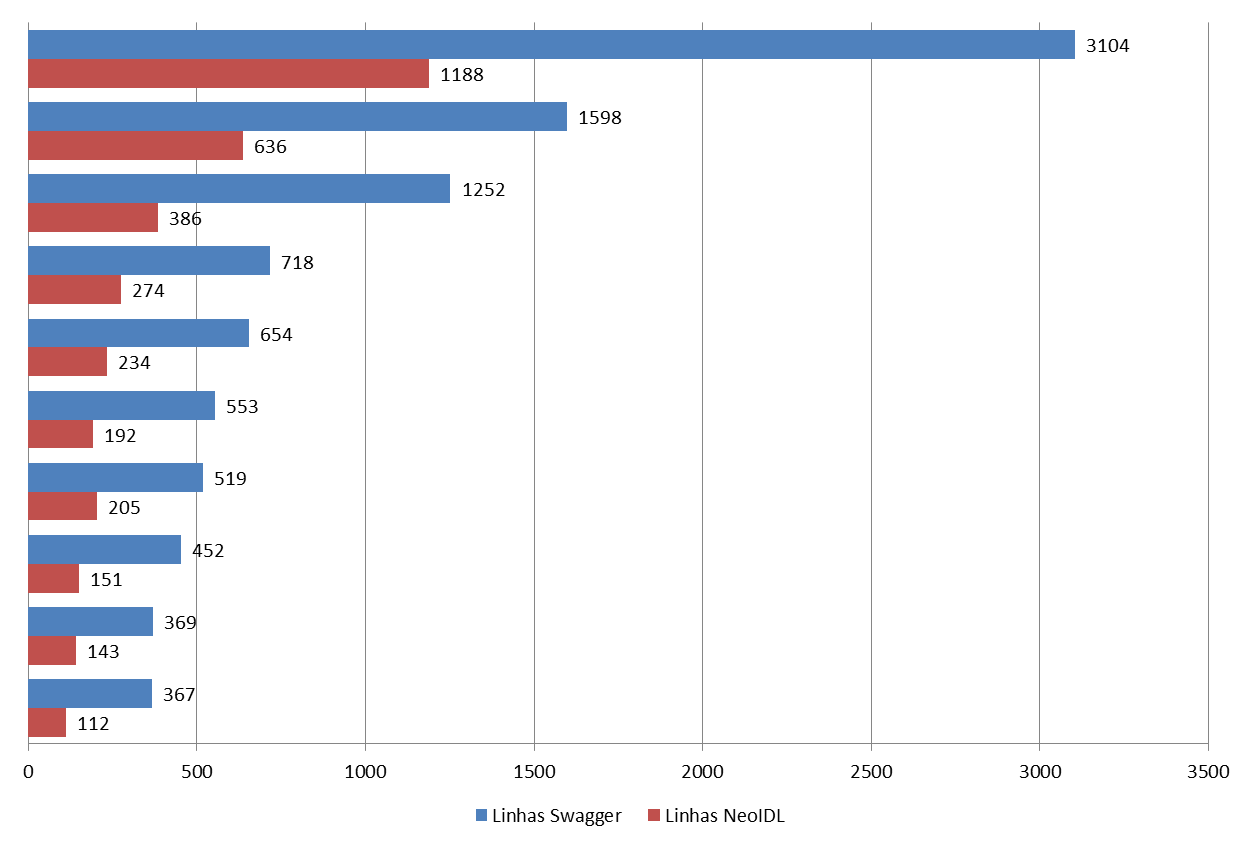
\includegraphics[width=8.5cm]{LinhasSwaggerNeoIDLMaiores.png}
\end{figure}

\end{frame}



\begin{frame}
\frametitle{Expressividade - Swagger x NeoIDL}

\begin{figure}[h] 
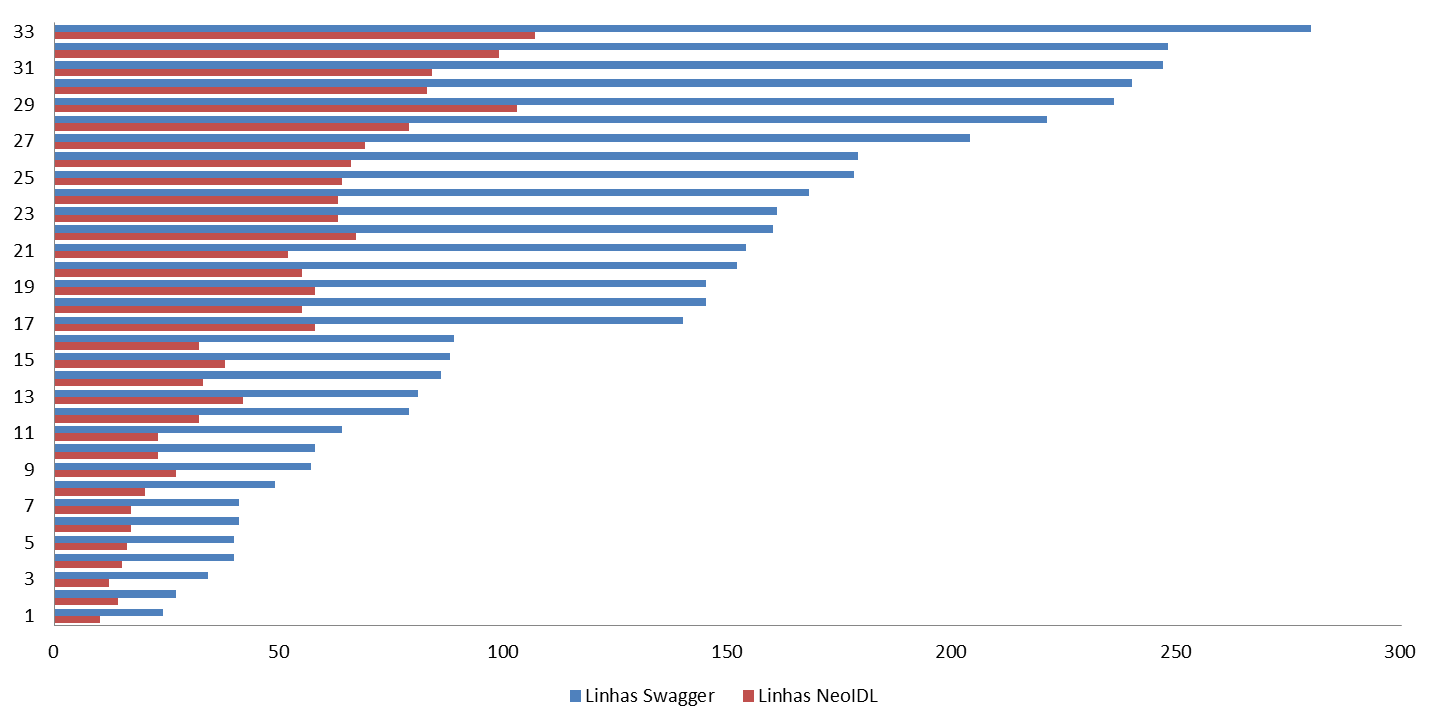
\includegraphics[width=10cm]{LinhasSwaggerNeoIDL.png}

\end{figure}

\end{frame}


\begin{frame}

Lucas Lima, et al. \emph{NeoIDL: A Domain Specific Language for Specifying REST
Contracts--- Detailed Design and Extended Evaluation}. International Journal of
Software Engineering and Knowledge Engineering. ({\bf submetido em 
Setembro de 2015}).

\end{frame}

\begin{frame}
\frametitle{Reuso}
\begin{itemize}
  \item 463 entidades diferentes declaradas nos 43 contratos
  \vskip0pt plus.5fill
  \pause
  \item 51 entidades com mais de uma ocorrência
  \vskip0pt plus.5fill
  \pause
  \item Casos críticos
  \begin{itemize}
	\item Ponto: 12 ocorrências
	\item Localizacao: 10 ocorrências
	\item Area: 6 ocorrências
	\item Item: 6 ocorrências
  \end{itemize}  
\end{itemize}

\end{frame}


\begin{frame}
\frametitle{Reuso}

\begin{figure}[htb]
\begin{tiny}
\lstinputlisting[language=NeoIDL,firstnumber=1]{Ponto.tex}
\end{tiny}
Entidade \emph{Ponto} em NeoIDL
\end{figure}

\begin{figure}[htb]
\begin{tiny}
\lstinputlisting[language=NeoIDL,firstnumber=1]{Area.tex}
\end{tiny}
Reuso da entidade \emph{Ponto} em NeoIDL	
\end{figure}

\end{frame}

% Slide com cronograma de atividades
\begin{frame}
\frametitle{Cronograma das próximas etapas} 

\begin{figure}[h] 
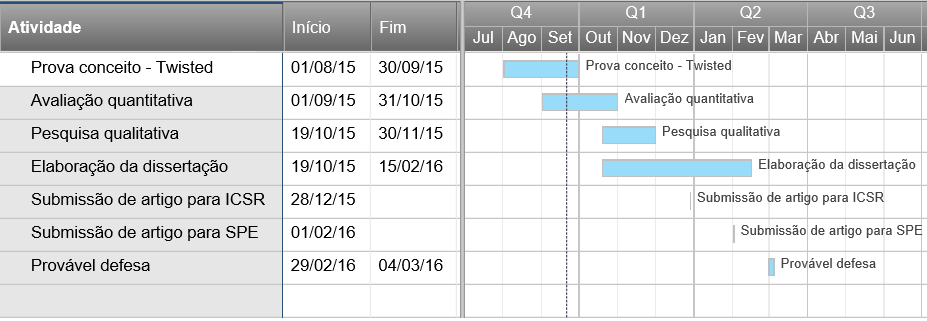
\includegraphics[width=10cm]{Gantt.png}

\end{figure}

\end{frame}

\begin{frame}

\begin{figure}[h]
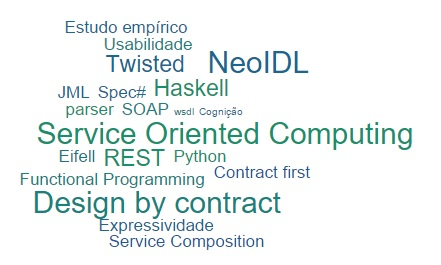
\includegraphics[width=7cm]{WordCloud.jpg}
\end{figure}


\end{frame}

\begin{frame}
\huge{Comentários}
\end{frame}

% Slide com título no final
\begin{frame}
\titlepage
\end{frame}

\end{document}
